\section{Quadratic Functions}

\begin{definition}[Quadratic Function]
    A \textbf{quadratic function} is a function of the form
    \[f(x) = ax^2 + bx + c\],
    where $a$, $b$ and $c$ are real numbers with $a \neq 0$. The domain of a quadratic function is $(-\infty, \infty)$
\end{definition}

\begin{definition}[Standard and General Form of Quadratic Functions]
    Suppose $f$ is a quadratic function.
    \begin{itemize}
        \item The \textbf{general form} of the quadratic function $f$ is $f(x) = ax^2 + bx + c$, where $a$, $b$ and $c$ are real numbers with $a \neq 0$
        \item The \textbf{standard form} of the quadratic function $f$ is $f(x)=a(x-h)^2 + k$, where $a$, $h$ and $k$ are real numbers with $a \neq 0$
    \end{itemize}
\end{definition}

\begin{definition}[Vertex Formula for Quadratics in Standard Form]
    For the qudratic function $f(x) = a(x-h)^2 + k$, where $a$, $h$ and $k$ are real numbers with $a \neq 0$, the vertex of the graph $y=f(x)$ is $(h,k)$
\end{definition}

\begin{definition}[Vertex Formulas for Quadratic Functions]
    Suppose $a$, $b$, $c$, $h$ and $k$ are real numbers with $a \neq 0$.
    \begin{itemize}
        \item If $f(x)=a(x-h)^2 + k$, the vertex of the graph of $y=f(x)$ is the point $(h,k)$
        \item If $f(x)=ax^2+bx+c$, the vertex of the graph $y=f(x)$ is the point $(-\frac{b}{2a}, f(-\frac{b}{2a}))$
    \end{itemize}
\end{definition}

\begin{definition}[The Quadratic Formula]
    If $a$, $b$ and $c$ are real numbers with $a \neq 0$, then the solutions to $ax^2 + bx + c = 0$ are
    \[
        x = \frac{-b \pm \sqrt{b^2 - 4ac}}{2a}
    \]
\end{definition}

\begin{definition}[Discriminant]
    If $a$, $b$ and $c$ are real numbers with $a \neq 0$, then the \textbf{discriminant} of the quadratic equation $ax^2 + bx + c = 0$ is the quantity $b^2 - 4ac$.
\end{definition}

\begin{definition}[Discriminant Trichotomy]
    Let $a$, $b$ and $c$ are real numbers with $a \neq 0$.
    \begin{itemize}
        \item If $b^2 - 4ac < 0$, the equation  $ax^2 + bx + c = 0$ has no real solutions.
        \item If $b^2 - 4ac = 0$, the equation  $ax^2 + bx + c = 0$ has exactly one real solutions.
        \item If $b^2 - 4ac > 0$, the equation  $ax^2 + bx + c = 0$ has exactly two real solutions.
    \end{itemize}
\end{definition}

\subsection{Exercises}
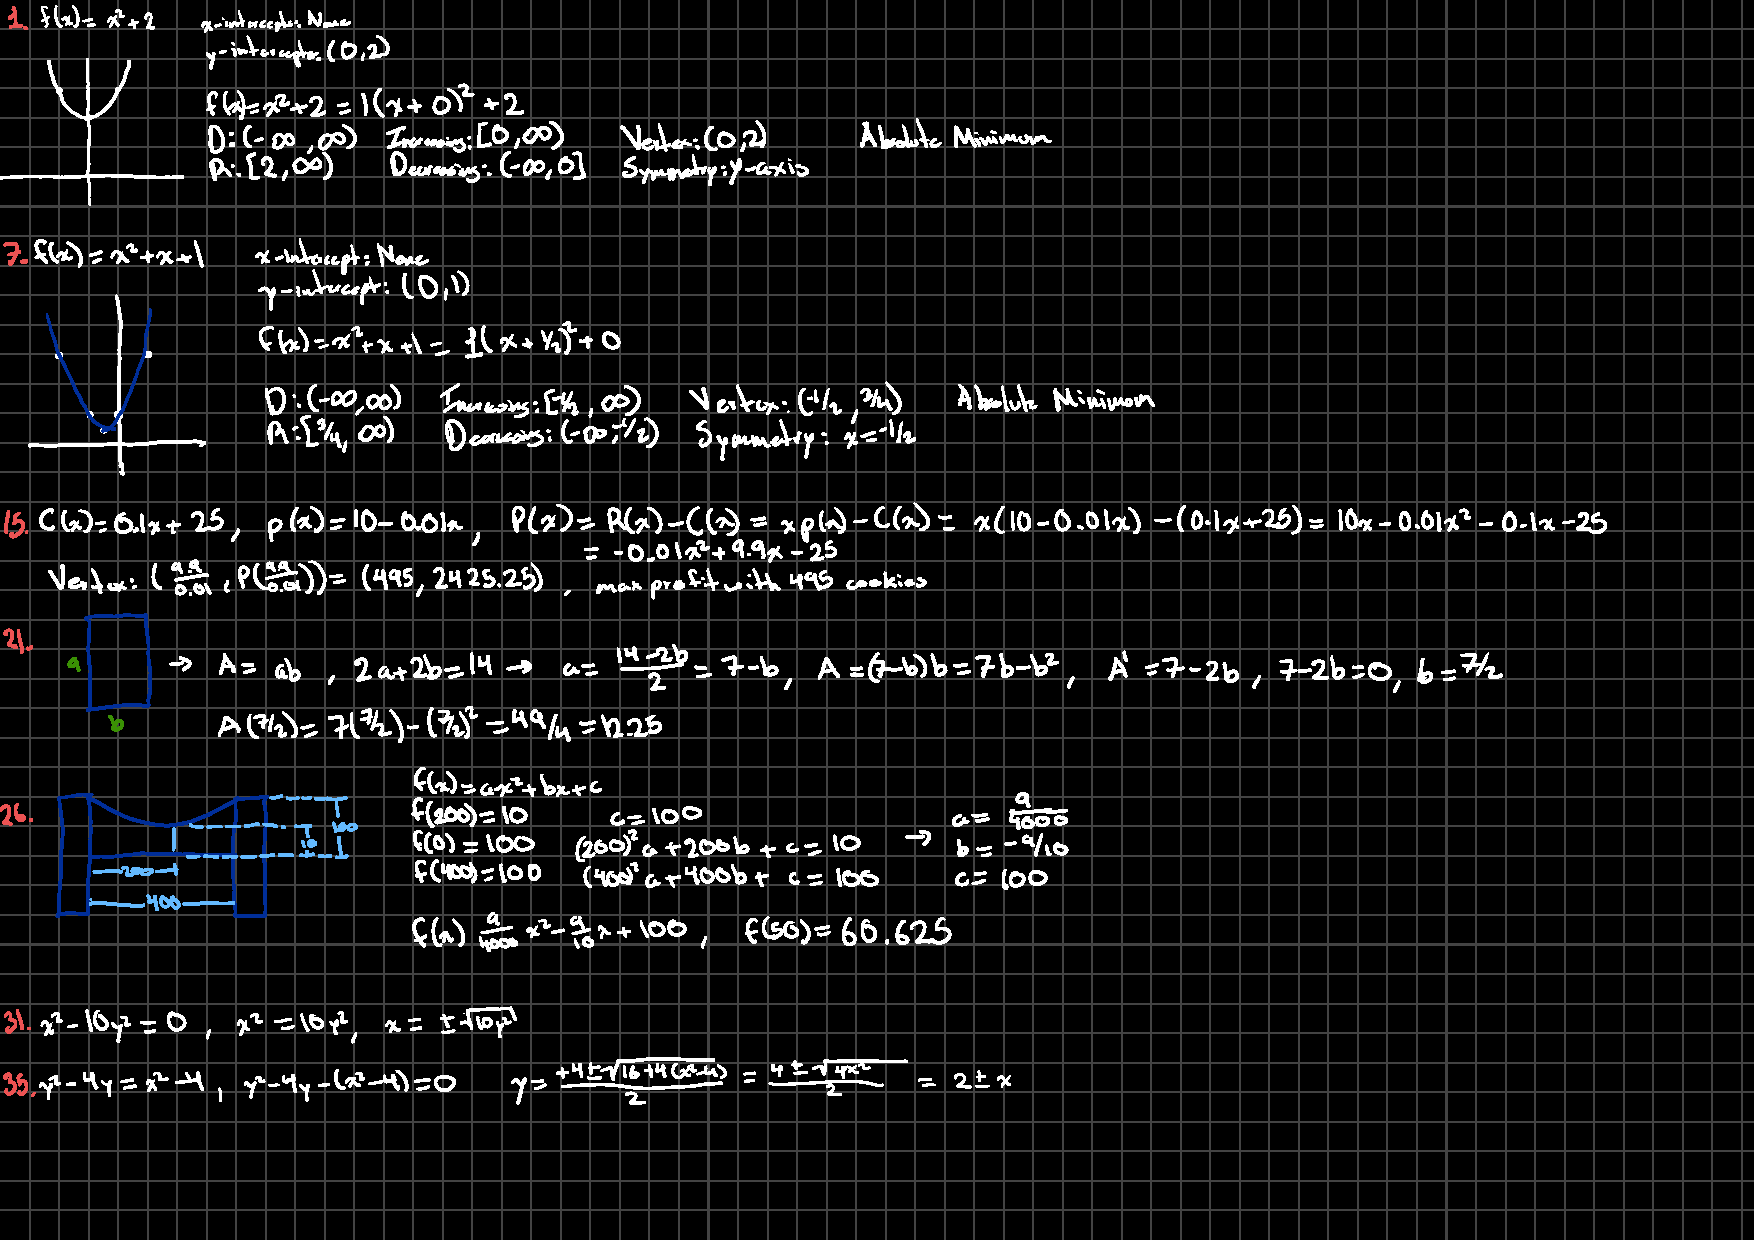
\includepdf[pages=-]{Exercises/02_Linear_and_Quadratic_Functions/03_Quadratic_Functions.pdf}
